\chapter{Testing Results}
Testing of the different revisions made, and trying to explain good and bad aspecs with this design.

\section{Waveform generator}
The ATtiny1617 provides the 125 kHz wave from that triggers the transistor to open and close the RLC circuit. This can be seen in figure \ref{fig:125khz:rise}

\begin{figure}[H]
    \centering
    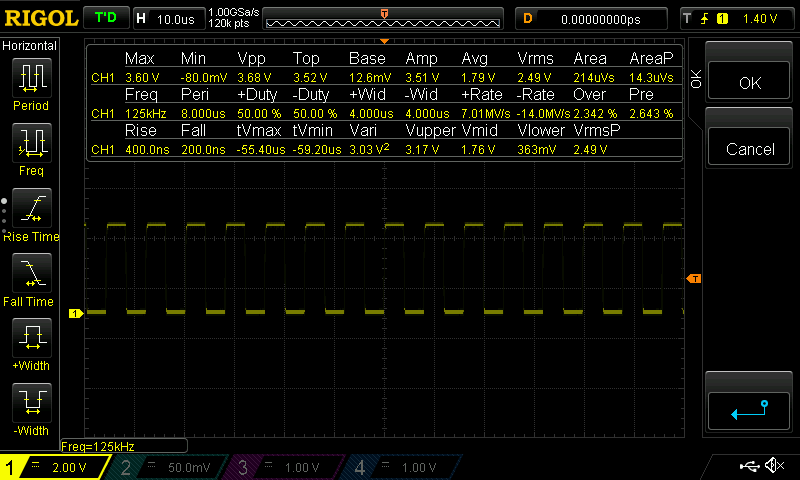
\includegraphics[width=\textwidth]{06_My_Testing_Results/figures/125khz_from_mcu/125_kHz_MCU.png}
    \caption{Waveform generated by the TCA module of the ATtiny1617}
    \label{fig:125khz:rise}
\end{figure}

\subsection{Setup-time for the reader}
The RFID tag can not be successfully read before the resonator has had the time to properly resonate. Due to the characteristics of this RLC circuit the rise time is measured to about 62$\mu$S. Given that one bit in the RFID tag is given as 64 periods on the 125kHz carrier, this means that the setup-time accounts for roughly 11\% of the first bit's readout time of the RFID tag. This amounts to about 7 periods as seen in figure \ref{fig:06:125khz:setup}.
\newline

It can then be reasoned that even though the circuit does not resonate perfectly instantaneously, we can start searching for start-of-frame immediately after calling the waveform initialization from the ATtiny1617 RFID reader.

\begin{figure}[H]
    \centering
    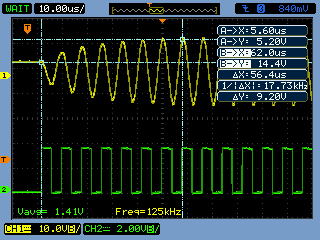
\includegraphics{06_My_Testing_Results/figures/125khz_from_mcu/resonator_startup.png}
    \caption{Setup time for the resonator in the RFID reader.}
    \label{fig:06:125khz:setup}
\end{figure}
\newpage
\section{Resonanse}
In figure \ref{fig:06:SinusVpp}
\begin{figure}[H]
    \centering
    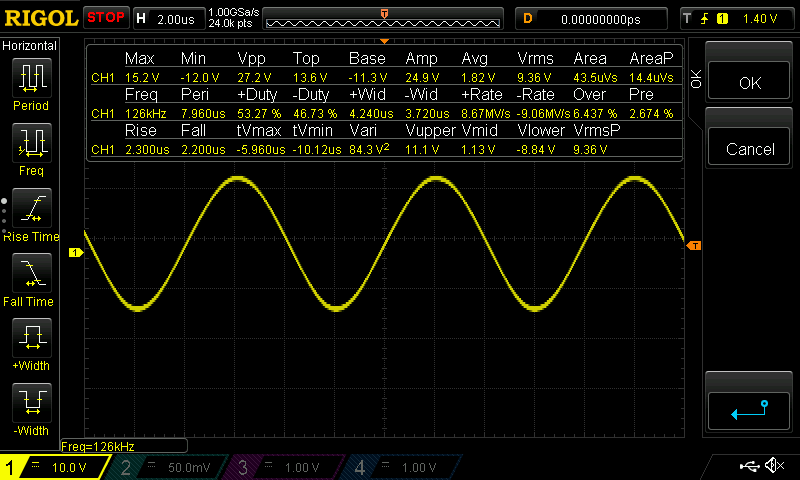
\includegraphics[width=\textwidth]{06_My_Testing_Results/figures/Out_from_transistor/125kHz_resonance_25Vpp.png}
    \caption{Sinus wave in the resonance circuit }
    \label{fig:06:SinusVpp}
\end{figure}

\section{Low pass filter}
The Low pass filter implemented shows its effect glamorously in figure \ref{fig:06:low_pass_full}. Here we see that the 125 kHz carry all but gone in the yellow signal. Granted one has to give up some rise-time for each flank, but the useful Vpp is still the same. By useful it is ment the difference between the lowest "high" and the highest "low" voltage. As the MCU is clocked at 8MHz, and sample time of the AC is far lower that the total length of a RFID bit, this has no effect on the readability of the tag. Furthermore for the same reason it does not change the read distance.

The difference in risetime can be seen in figure \ref{fig:06:low_pass_rise}.

\begin{figure}[H]
    \centering
    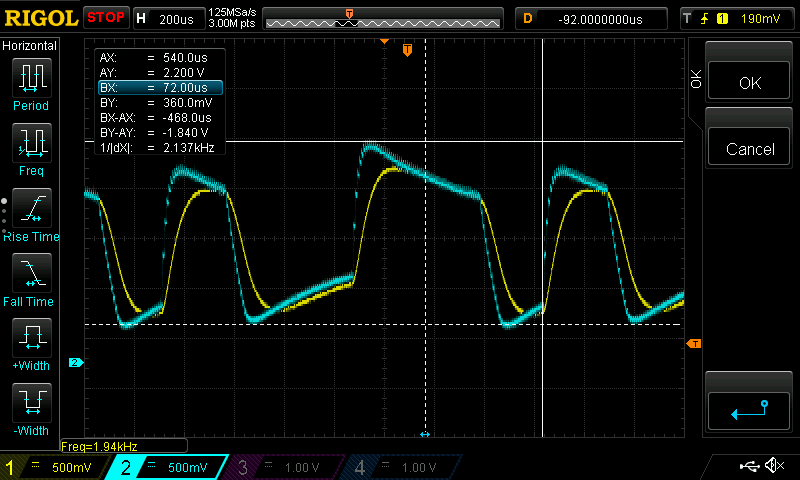
\includegraphics[width=\textwidth]{06_My_Testing_Results/figures/Low_pass_vs_no_low_pass/4_periods.png}
    \caption{Yellow line is after the Low Pass Filter, the blue is before}
    \label{fig:06:low_pass_full}
\end{figure}

\begin{figure}[H]
    \centering
    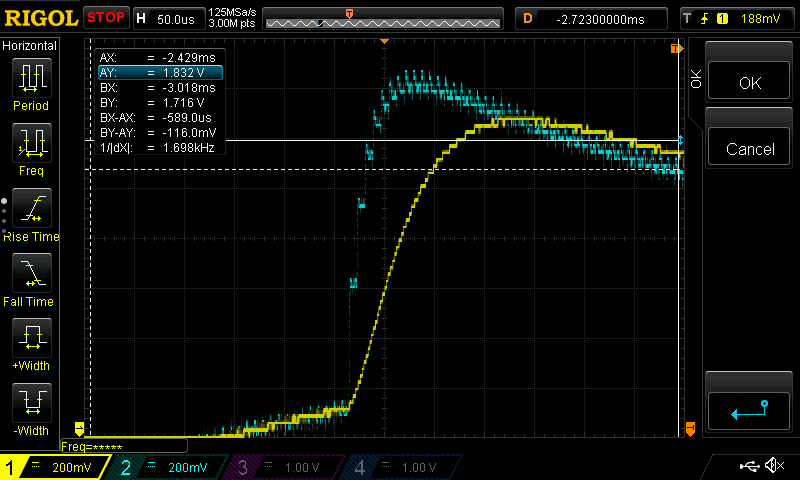
\includegraphics[width=\textwidth]{06_My_Testing_Results/figures/Low_pass_vs_no_low_pass/1_PERIOD.png}
    \caption{Risetime comparison of Low Pass vs no Low pass}
    \label{fig:06:low_pass_rise}
\end{figure}
\section{Interference with nearby coils}
Given that all of the 64 coils are tuned to the same frequency, they will affect each others electromagnetic fields. As stated in section \ref{sec:SuperPos} super position is the phenomena that causes this effect. If the two fields are slightly out of sync, the tag will not give a recognizable output as the field it is introduced to is not an uniform sine wave. This can be seen in figure \ref{fig:CoilSideBySide}. 

Here two coils are side by side, and appears to be out of sync, resulting in garbage data. Only one tag is introduced to the coil of interest, while the second coil is only active. This pattern will not be read as a valid tag.

\begin{figure}[H]
    \centering
    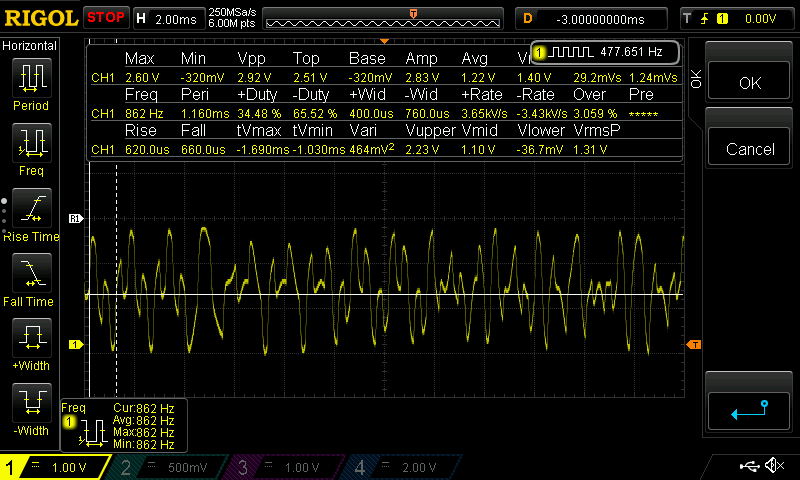
\includegraphics[width=\textwidth]{06_My_Testing_Results/figures/Several_readers_close/Besides_each_other.png}
    \caption{Two coils side by side}
    \label{fig:CoilSideBySide}
\end{figure}

A similar case where two coils are placed directly over each other with no tag inside their fields can be seen in figure \ref{fig:06:OnTopEO}. Here we observe a strange interference which does not appear to accrue periodically, at least not with the equipment at hand. 
For the most part the signal appears as a slightly distorted sine wave as seen on each side of the strange interference. Seeing as one of the coils in this system is a commercially available RFID reader meant for Windows applications, it might be so that it takes a break every now and then.

\begin{figure}[H]
    \centering
    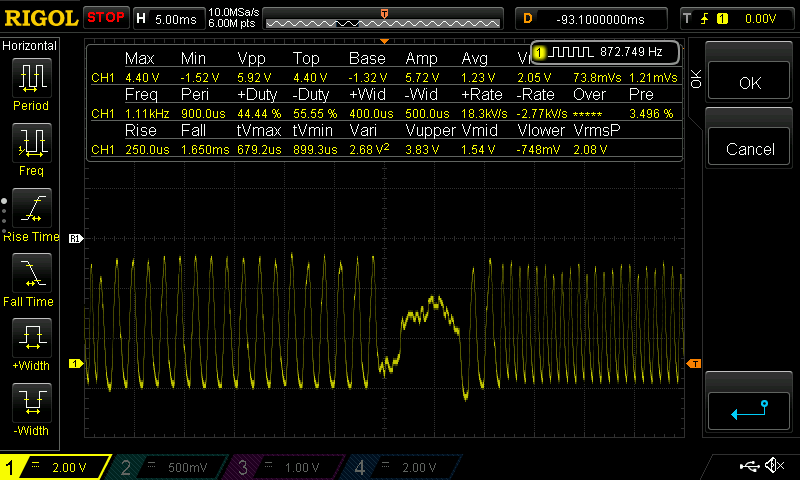
\includegraphics[width=\textwidth]{06_My_Testing_Results/figures/Several_readers_close/On_top_off_each_other.png}
    \caption{Two readers on top of each other}
    \label{fig:06:OnTopEO}
\end{figure}

As we move the coils further from each other, their fields interact less and less until the distortion is all but gone. At 3cm spacing we can see that a readable signal is obtainable. This is shown in figure \ref{fig:06:3cmAppart}

\begin{figure}[H]
    \centering
    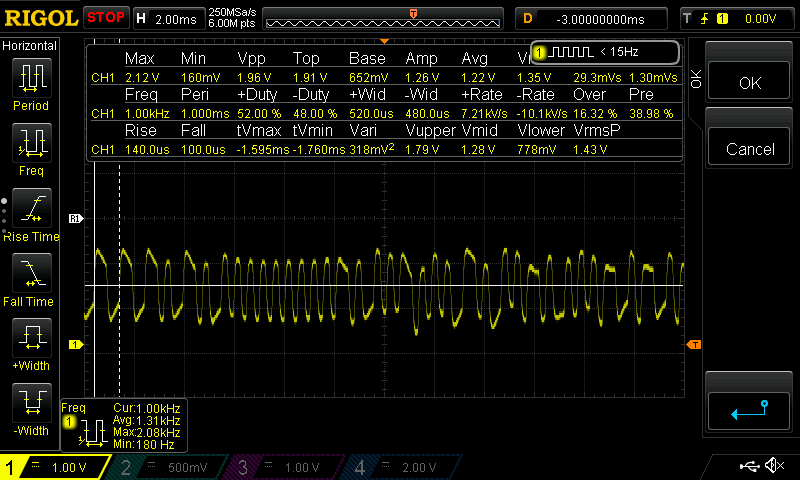
\includegraphics[width=\textwidth]{06_My_Testing_Results/figures/Several_readers_close/3_cm_spacing.png}
    \caption{Two active coils 3 cm from each other}
    \label{fig:06:3cmAppart}
\end{figure}







\section{Resistance in the resonance circuit}
The power used by thr circuit is heavily depended on 

\begin{figure}[H]
    \centering
    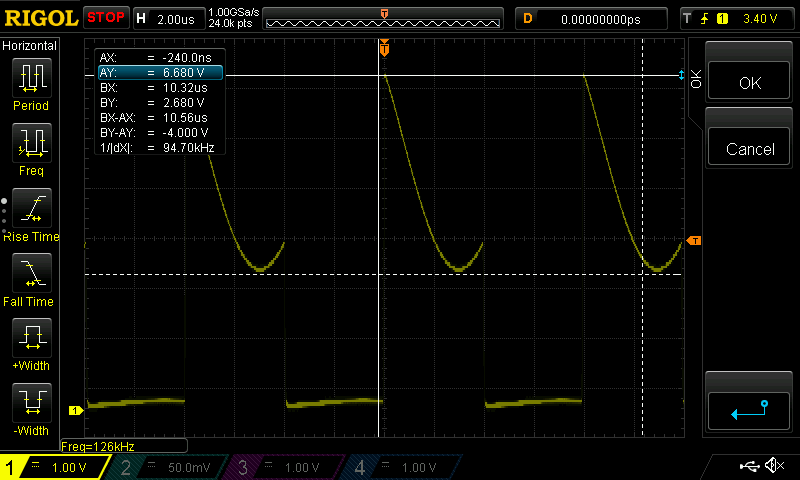
\includegraphics[width=\textwidth]{06_My_Testing_Results/figures/Out_from_transistor/125kHz_5V-125kHz_resonance_50ohm.png}
    \caption{Transistor side with 50 $\Omega$, here the voltage drop due to the driving of the coil is apparent}
    \label{fig:06:50Ohm}
\end{figure}
\begin{figure}[H]
    \centering
    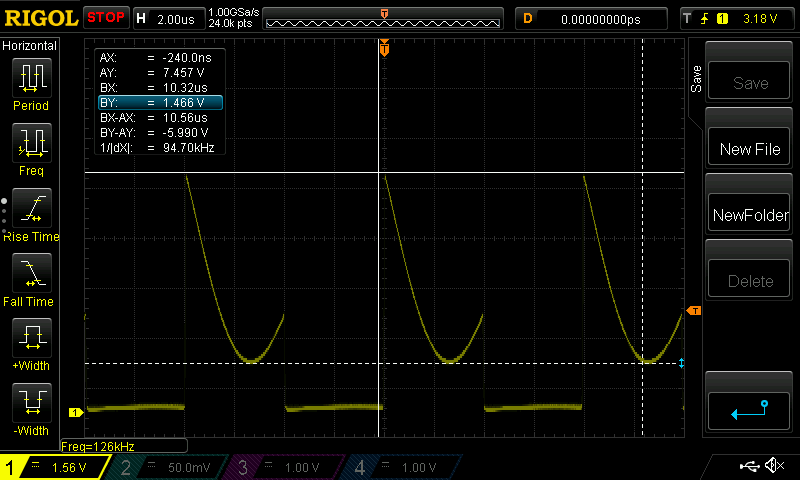
\includegraphics[width=\textwidth]{06_My_Testing_Results/figures/Out_from_transistor/125kHz_5V-125kHz_resonance_100ohm.png}
    \caption{Transistor side with 100 $\Omega$}
    \label{fig:06:100Ohm}
\end{figure}


\begin{figure}
    \centering
    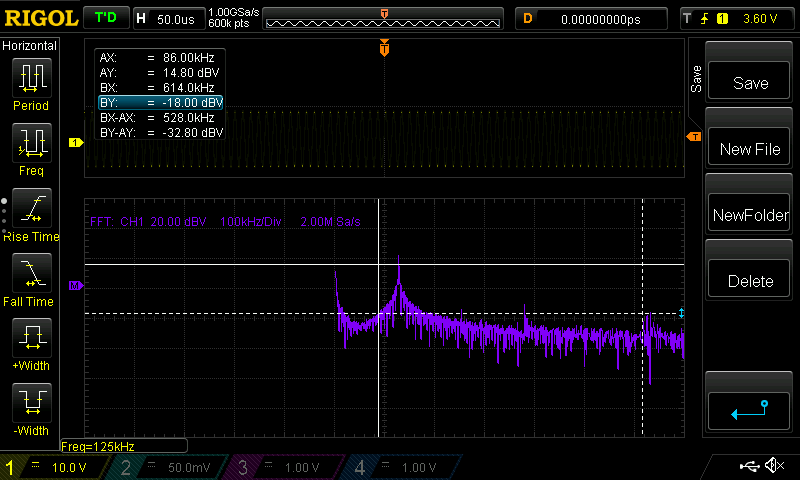
\includegraphics[width=\textwidth]{06_My_Testing_Results/figures/Out_from_transistor/harmony.png}
    \caption{The difference between the first and the third harmony is -18dB}
    \label{fig:06:Harmonies}
\end{figure}

\begin{figure}
    \centering
    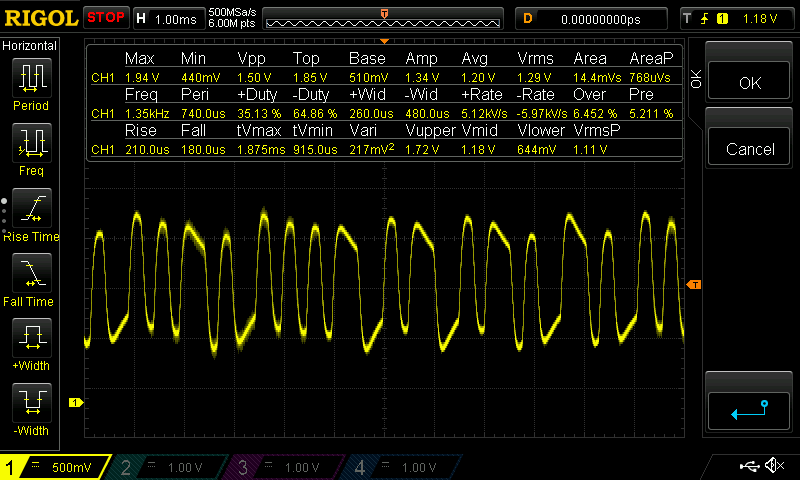
\includegraphics[width=\textwidth]{06_My_Testing_Results/figures/RFID_signal_with_different_resistance/100OHM.png}
    \caption{Tag readout with a 100 $\Omega$ resistor in the resonance circuit}
    \label{fig:06:TagReadout100Ohm}
\end{figure}

\begin{figure}
    \centering
    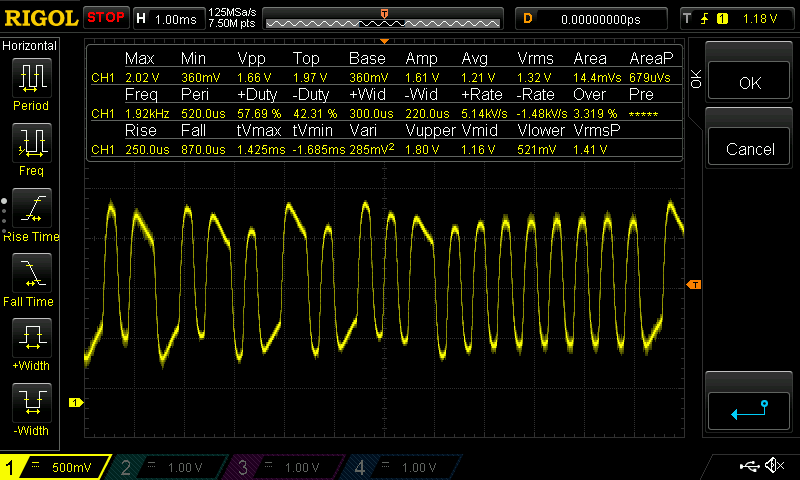
\includegraphics[width=\textwidth]{06_My_Testing_Results/figures/RFID_signal_with_different_resistance/50OHM.png}
    \caption{Tag readout with a 50 $\Omega$ resistor in the resonance circuit}
    \label{fig:06:TagReadout50Ohm}
\end{figure}

\begin{figure}
    \centering
    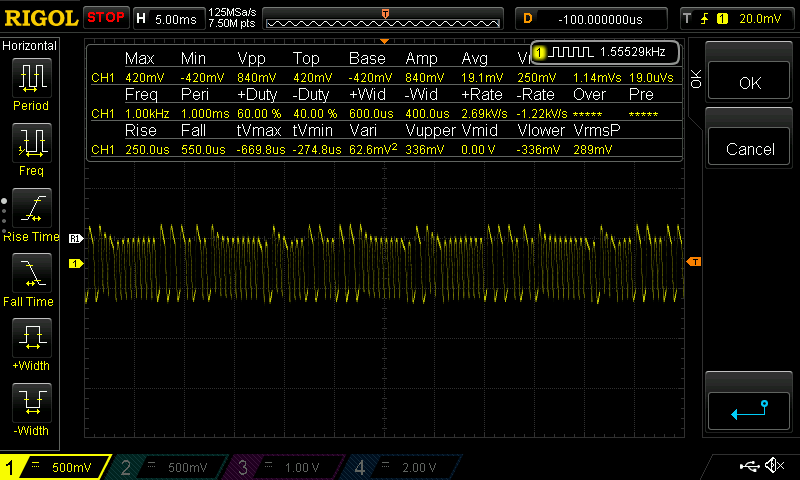
\includegraphics[width=\textwidth]{06_My_Testing_Results/figures/RFID_signal_with_different_resistance/Full_RFID_frame.png}
    \caption{Full frame view of the ID as seen by the AC}
    \label{fig:06:fullID}
\end{figure}


\begin{figure}
    \centering
    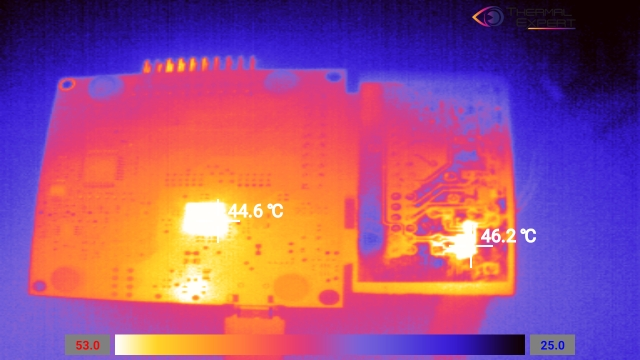
\includegraphics[width=\textwidth]{06_My_Testing_Results/figures/Heat_analysis/Heatmap_with_Xpro.jpg}
    \caption{Heat map showing a need for a higher grade resistor, here with the third revision of the RFID reader.}
    \label{fig:06:Heatmap1}
\end{figure}
\begin{figure}
    \centering
    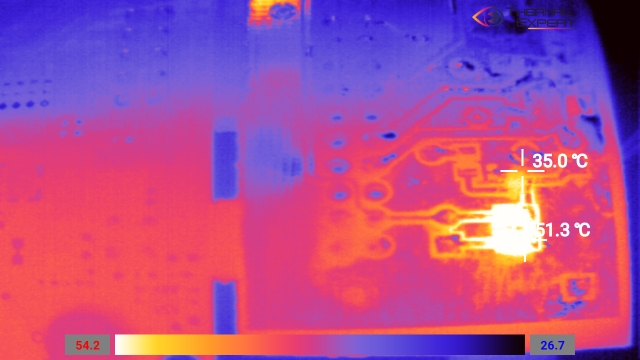
\includegraphics[width=\textwidth]{06_My_Testing_Results/figures/Heat_analysis/Heatmap_RFIDv3.jpg}
    \caption{Heat map suggesting a need for a higher grade resistor}
    \label{fig:06:Heatmap2}
\end{figure}

\section{Power Consumption}
